\documentclass{article}
\usepackage{makecell}
\usepackage{tikz}
\usetikzlibrary{arrows}
\usepackage{pgfplots}

\usetikzlibrary{external, patterns}

\tikzexternalize[prefix=out-]
\begin{document}

\centering
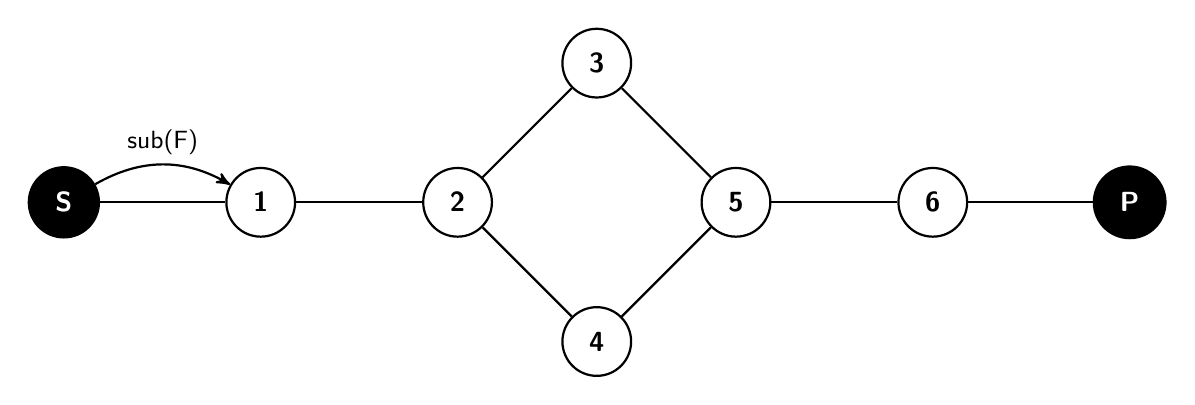
\begin{tikzpicture}[->,>=stealth',shorten >=0pt,auto,node distance=2.5cm, thick,main node/.style={circle,draw,font=\sffamily\bfseries, inner sep=0.2cm}, start node/.style={circle,draw,font=\sffamily\bfseries,text=white,fill=black, inner sep=0.2cm}]

  \node[start node] (S) [] {S};
  \node[main node] (1) [right of=S]{1};
  \node[main node] (2) [right of=1]{2};
  \node[main node] (3) [above right of=2]{3};
  \node[main node] (4) [below right of=2]{4};
  \node[main node] (5) [below right of=3]{5};
  \node[main node] (6) [right of=5]{6};
  \node[start node] (P) [right of=6]{P};

  \path[-,every node/.style={font=\sffamily\small}]
       (S) edge node {} (1)
       (1) edge node {} (2)
       (2) edge node {} (3)
       (2) edge node {} (4)
       (3) edge node {} (5)
       (4) edge node {} (5)
       (5) edge node {} (6)
       (6) edge node {} (P);

    \path[->,every node/.style={font=\sffamily\small}]
      (S) edge[bend left] node {sub(F)} (1)
    ;
    \path[->,every node/.style={font=\sffamily\small}, ultra thick]
    ;
\end{tikzpicture}

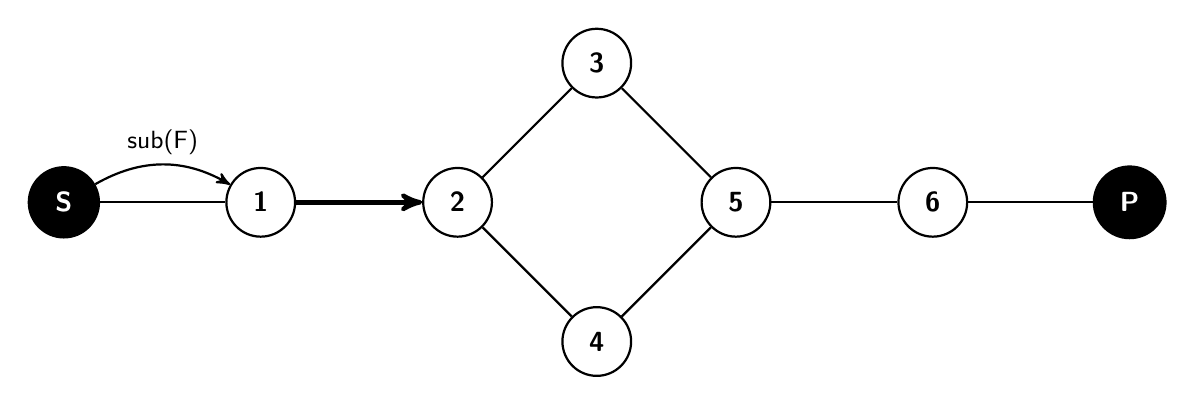
\begin{tikzpicture}[->,>=stealth',shorten >=0pt,auto,node distance=2.5cm, thick,main node/.style={circle,draw,font=\sffamily\bfseries, inner sep=0.2cm}, start node/.style={circle,draw,font=\sffamily\bfseries,text=white,fill=black, inner sep=0.2cm}]

  \node[start node] (S) [] {S};
  \node[main node] (1) [right of=S]{1};
  \node[main node] (2) [right of=1]{2};
  \node[main node] (3) [above right of=2]{3};
  \node[main node] (4) [below right of=2]{4};
  \node[main node] (5) [below right of=3]{5};
  \node[main node] (6) [right of=5]{6};
  \node[start node] (P) [right of=6]{P};

  \path[-,every node/.style={font=\sffamily\small}]
       (S) edge node {} (1)
       (1) edge node {} (2)
       (2) edge node {} (3)
       (2) edge node {} (4)
       (3) edge node {} (5)
       (4) edge node {} (5)
       (5) edge node {} (6)
       (6) edge node {} (P);

    \path[->,every node/.style={font=\sffamily\small}]
      (S) edge[bend left] node {sub(F)} (1)
    ;
    \path[->,every node/.style={font=\sffamily\small}, ultra thick]
      (1) edge node {} (2)
    ;
\end{tikzpicture}


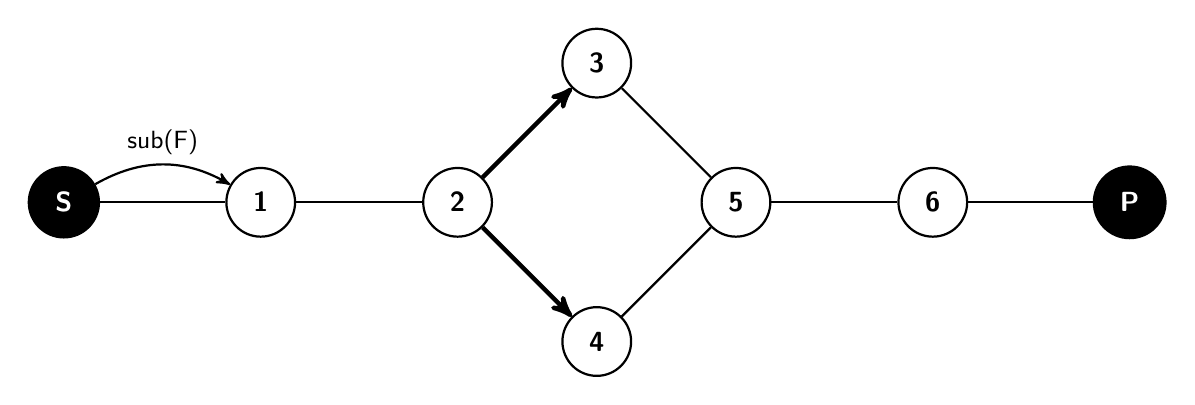
\begin{tikzpicture}[->,>=stealth',shorten >=0pt,auto,node distance=2.5cm, thick,main node/.style={circle,draw,font=\sffamily\bfseries, inner sep=0.2cm}, start node/.style={circle,draw,font=\sffamily\bfseries,text=white,fill=black, inner sep=0.2cm}]

  \node[start node] (S) [] {S};
  \node[main node] (1) [right of=S]{1};
  \node[main node] (2) [right of=1]{2};
  \node[main node] (3) [above right of=2]{3};
  \node[main node] (4) [below right of=2]{4};
  \node[main node] (5) [below right of=3]{5};
  \node[main node] (6) [right of=5]{6};
  \node[start node] (P) [right of=6]{P};

  \path[-,every node/.style={font=\sffamily\small}]
       (S) edge node {} (1)
       (1) edge node {} (2)
       (2) edge node {} (3)
       (2) edge node {} (4)
       (3) edge node {} (5)
       (4) edge node {} (5)
       (5) edge node {} (6)
       (6) edge node {} (P);

    \path[->,every node/.style={font=\sffamily\small}]
      (S) edge[bend left] node {sub(F)} (1)
    ;
    \path[->,every node/.style={font=\sffamily\small}, ultra thick]
      (2) edge node {} (3)
      (2) edge node {} (4)
    ;
\end{tikzpicture}

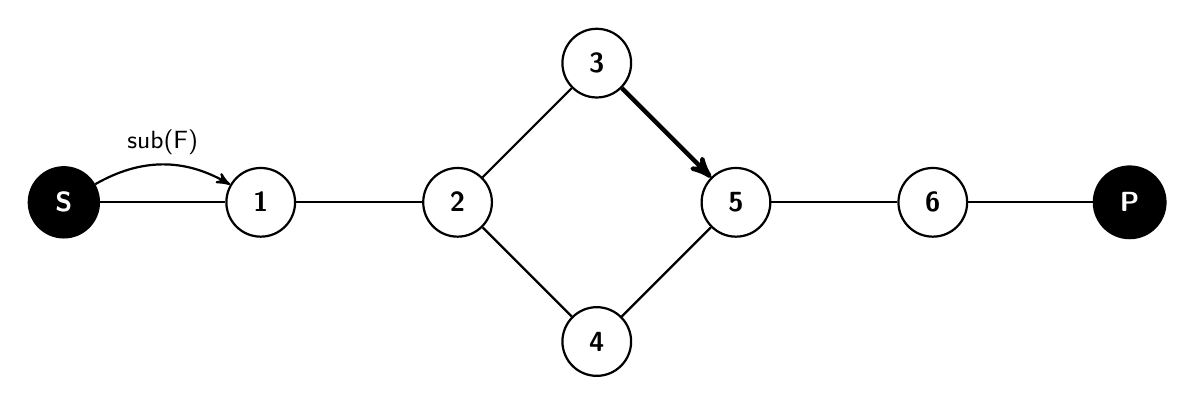
\begin{tikzpicture}[->,>=stealth',shorten >=0pt,auto,node distance=2.5cm, thick,main node/.style={circle,draw,font=\sffamily\bfseries, inner sep=0.2cm}, start node/.style={circle,draw,font=\sffamily\bfseries,text=white,fill=black, inner sep=0.2cm}]

  \node[start node] (S) [] {S};
  \node[main node] (1) [right of=S]{1};
  \node[main node] (2) [right of=1]{2};
  \node[main node] (3) [above right of=2]{3};
  \node[main node] (4) [below right of=2]{4};
  \node[main node] (5) [below right of=3]{5};
  \node[main node] (6) [right of=5]{6};
  \node[start node] (P) [right of=6]{P};

  \path[-,every node/.style={font=\sffamily\small}]
       (S) edge node {} (1)
       (1) edge node {} (2)
       (2) edge node {} (3)
       (2) edge node {} (4)
       (3) edge node {} (5)
       (4) edge node {} (5)
       (5) edge node {} (6)
       (6) edge node {} (P);

    \path[->,every node/.style={font=\sffamily\small}]
      (S) edge[bend left] node {sub(F)} (1)
    ;
    \path[->,every node/.style={font=\sffamily\small}, ultra thick]
      (3) edge node {} (5)
    ;
\end{tikzpicture}

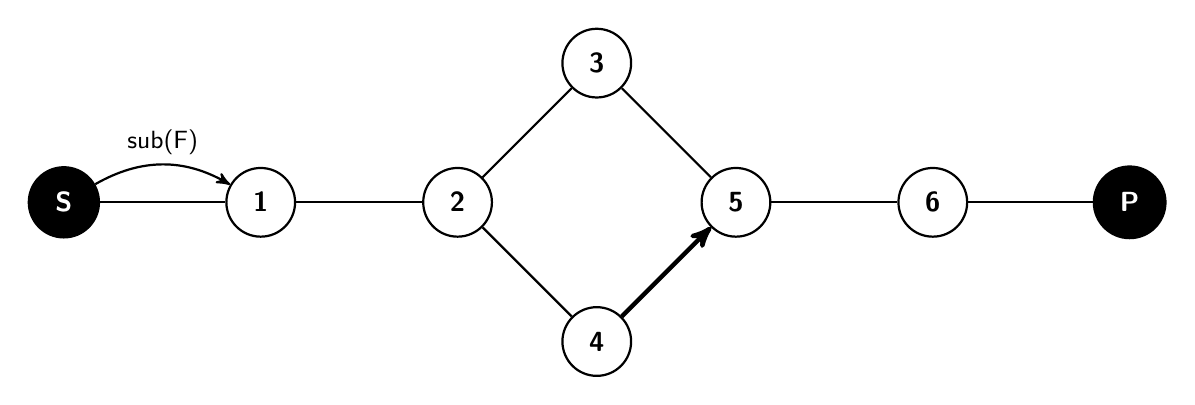
\begin{tikzpicture}[->,>=stealth',shorten >=0pt,auto,node distance=2.5cm, thick,main node/.style={circle,draw,font=\sffamily\bfseries, inner sep=0.2cm}, start node/.style={circle,draw,font=\sffamily\bfseries,text=white,fill=black, inner sep=0.2cm}]

  \node[start node] (S) [] {S};
  \node[main node] (1) [right of=S]{1};
  \node[main node] (2) [right of=1]{2};
  \node[main node] (3) [above right of=2]{3};
  \node[main node] (4) [below right of=2]{4};
  \node[main node] (5) [below right of=3]{5};
  \node[main node] (6) [right of=5]{6};
  \node[start node] (P) [right of=6]{P};

  \path[-,every node/.style={font=\sffamily\small}]
       (S) edge node {} (1)
       (1) edge node {} (2)
       (2) edge node {} (3)
       (2) edge node {} (4)
       (3) edge node {} (5)
       (4) edge node {} (5)
       (5) edge node {} (6)
       (6) edge node {} (P);

    \path[->,every node/.style={font=\sffamily\small}]
      (S) edge[bend left] node {sub(F)} (1)
    ;
    \path[->,every node/.style={font=\sffamily\small}, ultra thick]
      (4) edge node {} (5)
    ;
\end{tikzpicture}

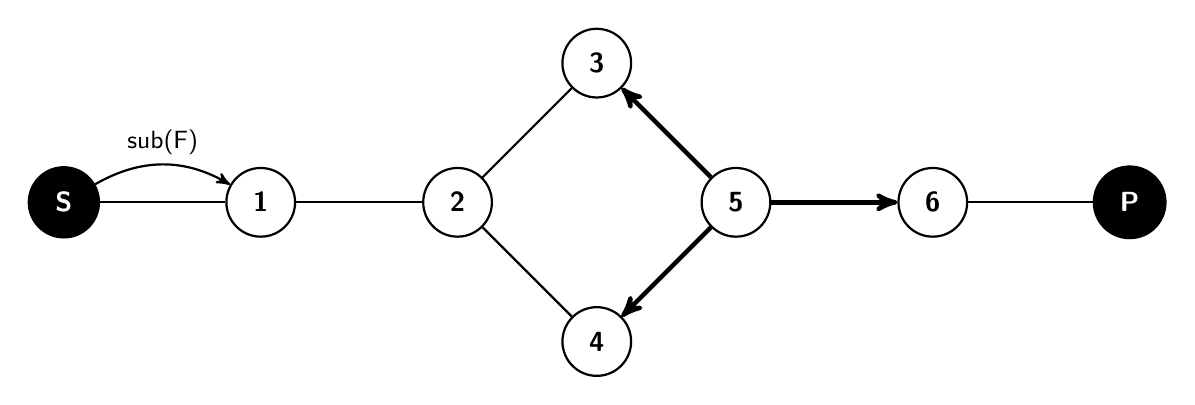
\begin{tikzpicture}[->,>=stealth',shorten >=0pt,auto,node distance=2.5cm, thick,main node/.style={circle,draw,font=\sffamily\bfseries, inner sep=0.2cm}, start node/.style={circle,draw,font=\sffamily\bfseries,text=white,fill=black, inner sep=0.2cm}]

  \node[start node] (S) [] {S};
  \node[main node] (1) [right of=S]{1};
  \node[main node] (2) [right of=1]{2};
  \node[main node] (3) [above right of=2]{3};
  \node[main node] (4) [below right of=2]{4};
  \node[main node] (5) [below right of=3]{5};
  \node[main node] (6) [right of=5]{6};
  \node[start node] (P) [right of=6]{P};

  \path[-,every node/.style={font=\sffamily\small}]
       (S) edge node {} (1)
       (1) edge node {} (2)
       (2) edge node {} (3)
       (2) edge node {} (4)
       (3) edge node {} (5)
       (4) edge node {} (5)
       (5) edge node {} (6)
       (6) edge node {} (P);

    \path[->,every node/.style={font=\sffamily\small}]
      (S) edge[bend left] node {sub(F)} (1)
    ;
    \path[->,every node/.style={font=\sffamily\small}, ultra thick]
      (5) edge node {} (4)
      (5) edge node {} (3)
      (5) edge node {} (6)
    ;
\end{tikzpicture}

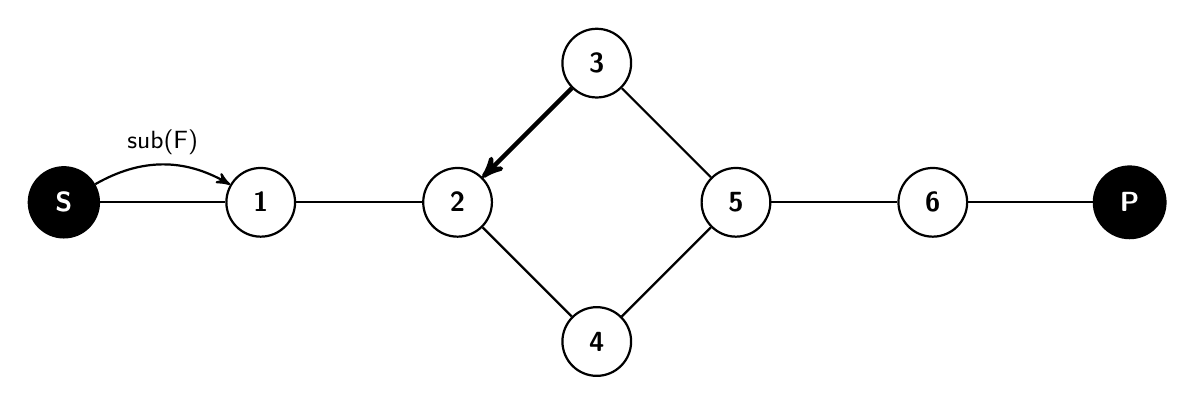
\begin{tikzpicture}[->,>=stealth',shorten >=0pt,auto,node distance=2.5cm, thick,main node/.style={circle,draw,font=\sffamily\bfseries, inner sep=0.2cm}, start node/.style={circle,draw,font=\sffamily\bfseries,text=white,fill=black, inner sep=0.2cm}]

  \node[start node] (S) [] {S};
  \node[main node] (1) [right of=S]{1};
  \node[main node] (2) [right of=1]{2};
  \node[main node] (3) [above right of=2]{3};
  \node[main node] (4) [below right of=2]{4};
  \node[main node] (5) [below right of=3]{5};
  \node[main node] (6) [right of=5]{6};
  \node[start node] (P) [right of=6]{P};

  \path[-,every node/.style={font=\sffamily\small}]
       (S) edge node {} (1)
       (1) edge node {} (2)
       (2) edge node {} (3)
       (2) edge node {} (4)
       (3) edge node {} (5)
       (4) edge node {} (5)
       (5) edge node {} (6)
       (6) edge node {} (P);

    \path[->,every node/.style={font=\sffamily\small}]
      (S) edge[bend left] node {sub(F)} (1)
    ;
    \path[->,every node/.style={font=\sffamily\small}, ultra thick]
      (3) edge node {} (2)
    ;
\end{tikzpicture}

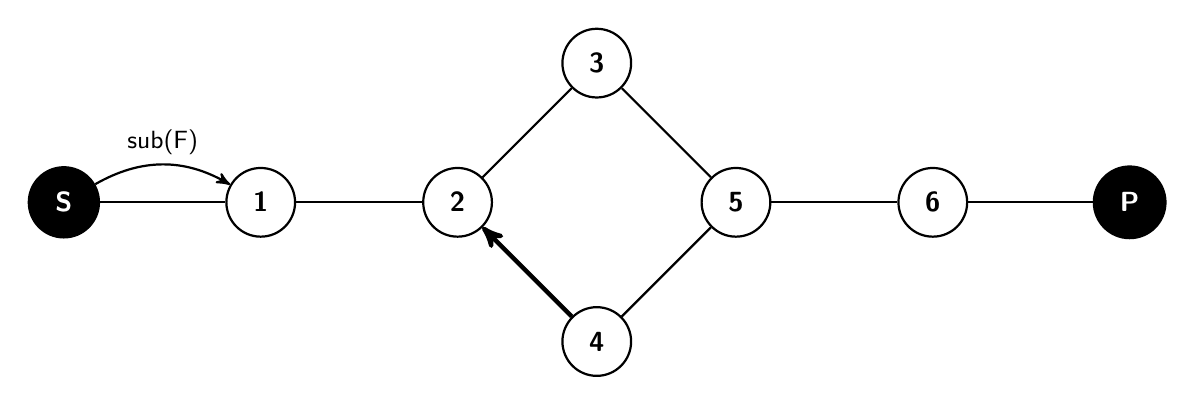
\begin{tikzpicture}[->,>=stealth',shorten >=0pt,auto,node distance=2.5cm, thick,main node/.style={circle,draw,font=\sffamily\bfseries, inner sep=0.2cm}, start node/.style={circle,draw,font=\sffamily\bfseries,text=white,fill=black, inner sep=0.2cm}]

  \node[start node] (S) [] {S};
  \node[main node] (1) [right of=S]{1};
  \node[main node] (2) [right of=1]{2};
  \node[main node] (3) [above right of=2]{3};
  \node[main node] (4) [below right of=2]{4};
  \node[main node] (5) [below right of=3]{5};
  \node[main node] (6) [right of=5]{6};
  \node[start node] (P) [right of=6]{P};

  \path[-,every node/.style={font=\sffamily\small}]
       (S) edge node {} (1)
       (1) edge node {} (2)
       (2) edge node {} (3)
       (2) edge node {} (4)
       (3) edge node {} (5)
       (4) edge node {} (5)
       (5) edge node {} (6)
       (6) edge node {} (P);

    \path[->,every node/.style={font=\sffamily\small}]
      (S) edge[bend left] node {sub(F)} (1)
    ;
    \path[->,every node/.style={font=\sffamily\small}, ultra thick]
      (4) edge node {} (2)
    ;
\end{tikzpicture}

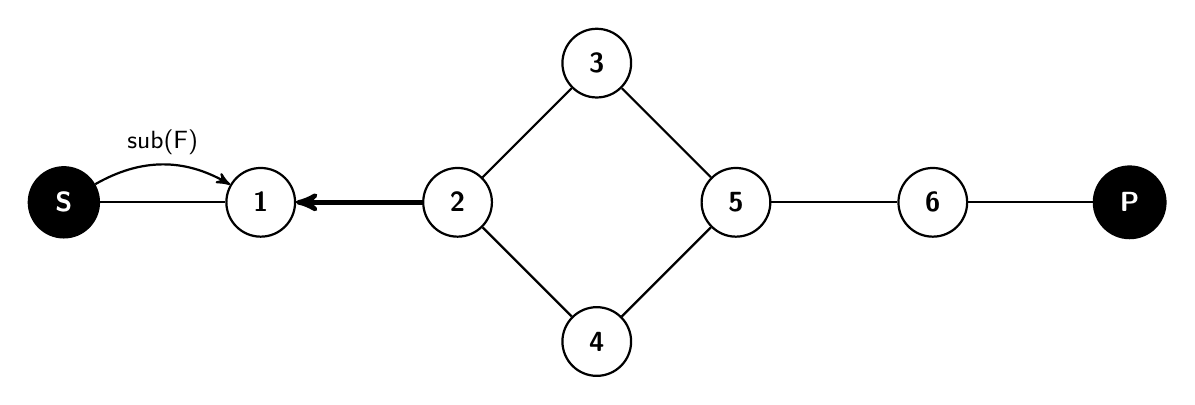
\begin{tikzpicture}[->,>=stealth',shorten >=0pt,auto,node distance=2.5cm, thick,main node/.style={circle,draw,font=\sffamily\bfseries, inner sep=0.2cm}, start node/.style={circle,draw,font=\sffamily\bfseries,text=white,fill=black, inner sep=0.2cm}]

  \node[start node] (S) [] {S};
  \node[main node] (1) [right of=S]{1};
  \node[main node] (2) [right of=1]{2};
  \node[main node] (3) [above right of=2]{3};
  \node[main node] (4) [below right of=2]{4};
  \node[main node] (5) [below right of=3]{5};
  \node[main node] (6) [right of=5]{6};
  \node[start node] (P) [right of=6]{P};

  \path[-,every node/.style={font=\sffamily\small}]
       (S) edge node {} (1)
       (1) edge node {} (2)
       (2) edge node {} (3)
       (2) edge node {} (4)
       (3) edge node {} (5)
       (4) edge node {} (5)
       (5) edge node {} (6)
       (6) edge node {} (P);

    \path[->,every node/.style={font=\sffamily\small}]
      (S) edge[bend left] node {sub(F)} (1)
    ;
    \path[->,every node/.style={font=\sffamily\small}, ultra thick]
      (2) edge node {} (1)
    ;
\end{tikzpicture}

\end{document}
